% !TeX encoding=utf8
% !TeX spellcheck = en-US

\chapter{Evaluation}

\section{Testing the visualisation method}

The visualising methods is the main work of the project, thus, comparing each method and discovering the problems of the methods are important.

\subsection{Cross in planar map}
The most essential feature of planar graph is no cross inside of the graph. Therefore, this is the primary assessment criterion for the methods when generate a planar map.

\begin{figure}[htb]
    \centering
    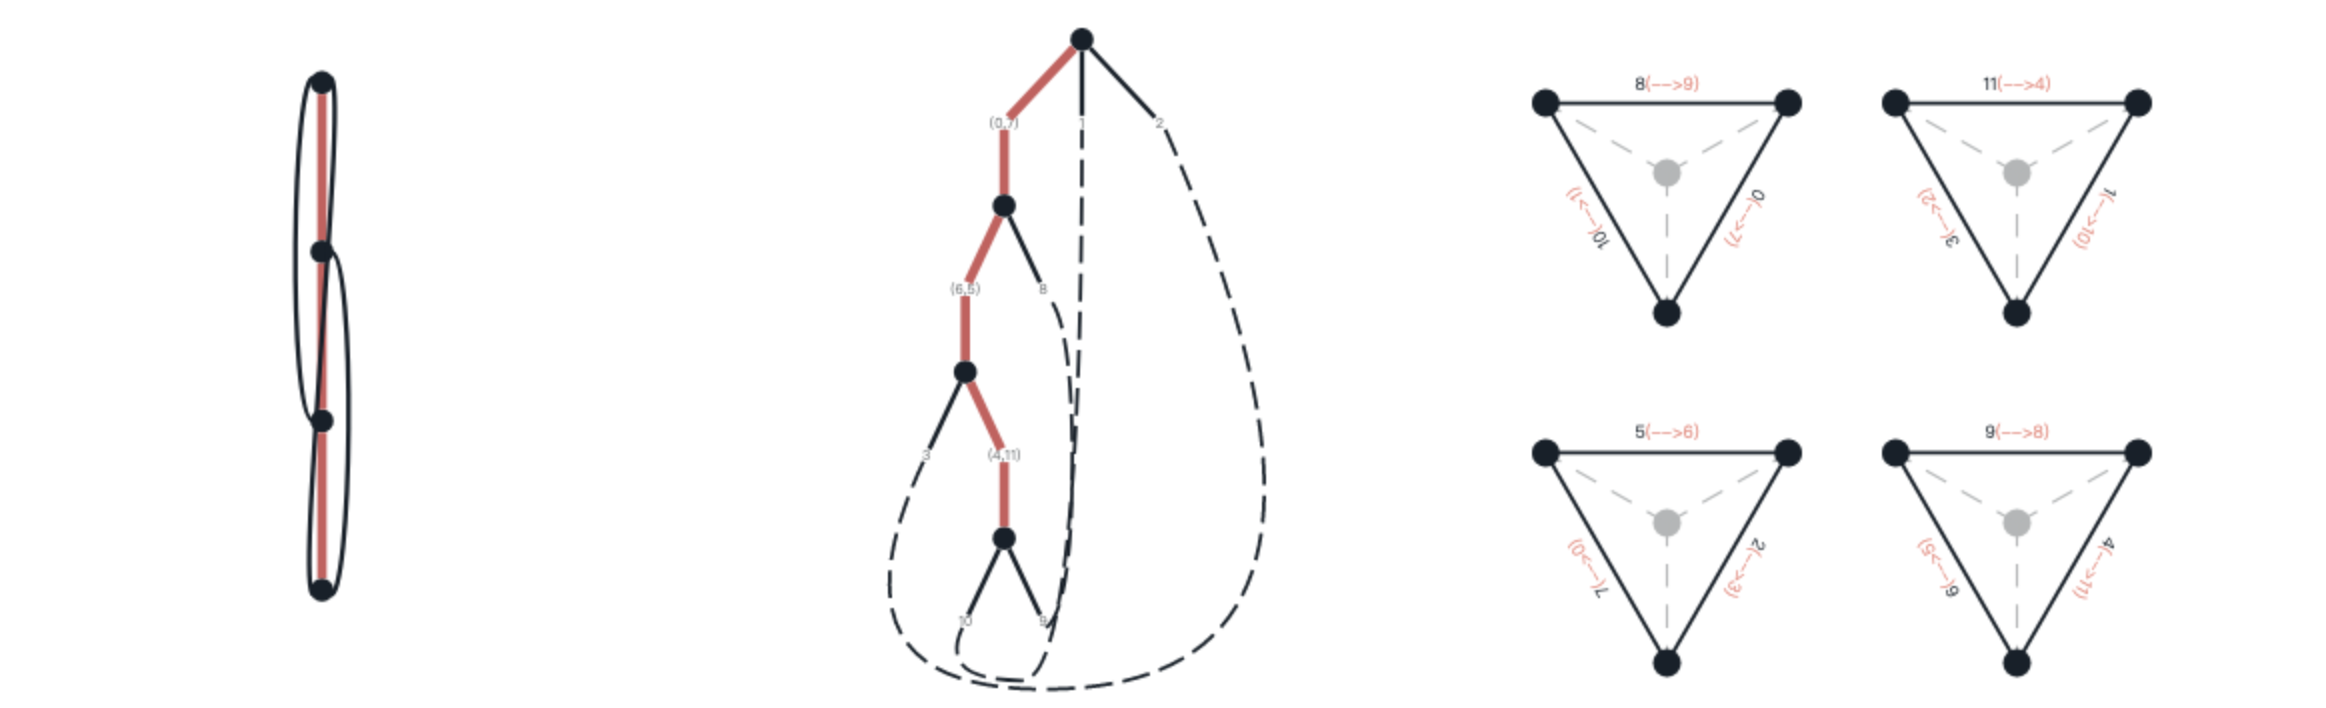
\includegraphics[width=0.8\textwidth]{../../image/cross1.png}
    \caption{Results of planar Tetrahedron.}
    \label{fig:figures:cross1}
  \end{figure}

  The \cref{fig:figures:cross1} shows a simple planar map called planar Tetrahedron, it is obvious that the last two methods work well and avoiding the cross successfully, though the gap between lines in the second method is too narrow. However, the first approach cannot handle the problem completely.

  \begin{figure}[htb]
    \centering
    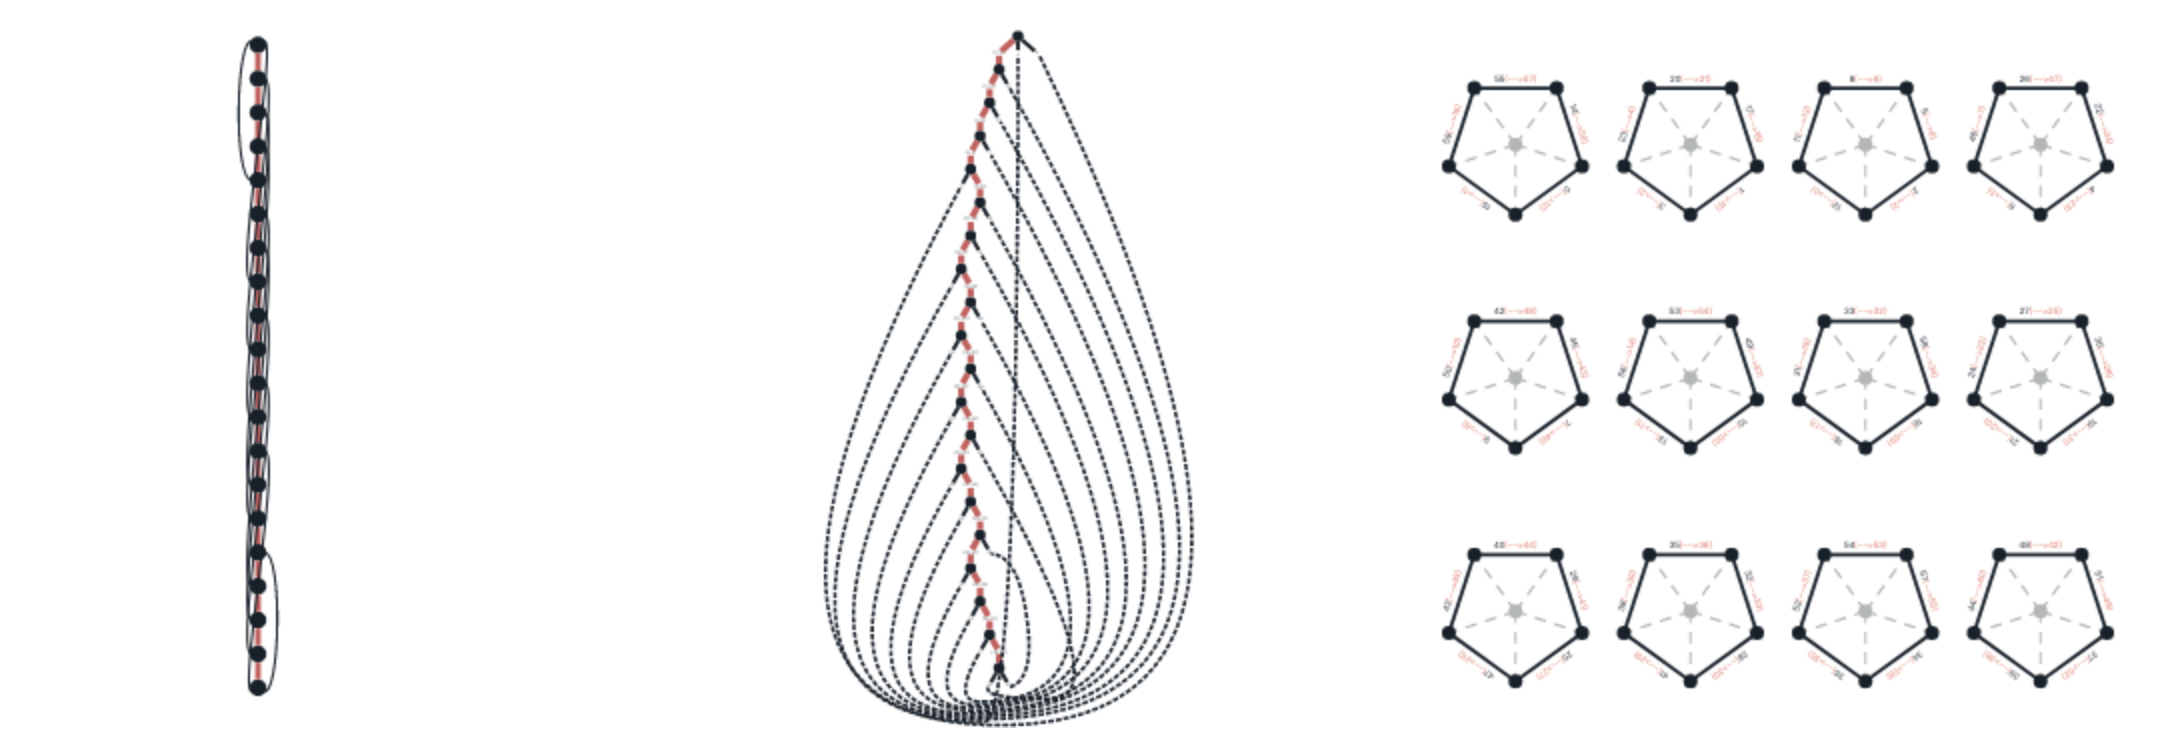
\includegraphics[width=0.8\textwidth]{../../image/cross2.png}
    \caption{Results of dodecahedron graph.}
    \label{fig:figures:cross2}
  \end{figure}
  The solutions of a larger map for dodecahedron graph display in the \cref{fig:figures:cross2}. For this map, the first map becomes mass and unclear, and the last method is still tidy without cross. The second method, however, is not up to standard because the cross appear in the two of curves.
  \begin{figure}[htb]
    \centering
    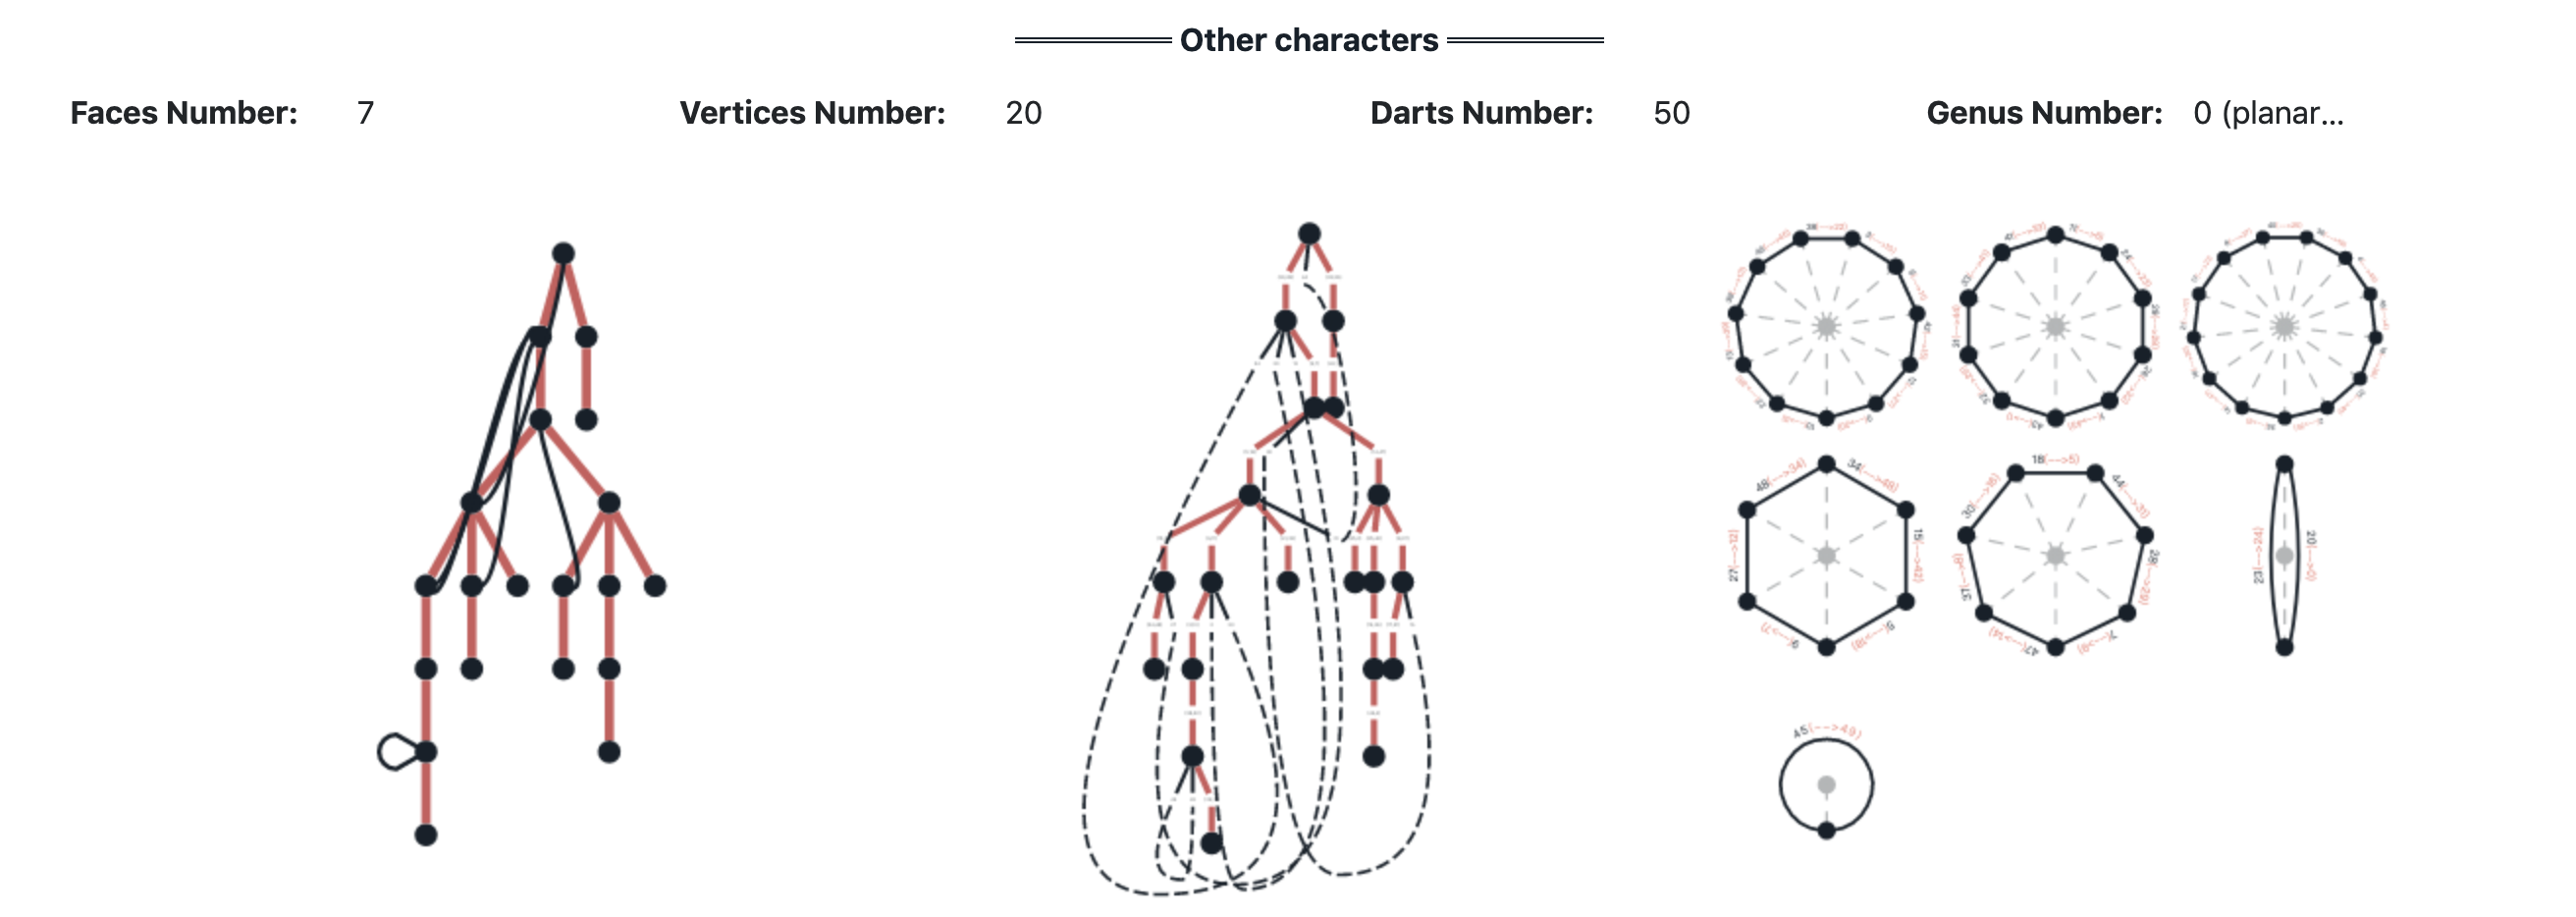
\includegraphics[width=0.8\textwidth]{../../image/randomplanar.png}
    \caption{Results of a random planar map.}
    \label{fig:figures:randomplanar}
  \end{figure}
  \newpage
  Besides the example, the \cref{fig:figures:randomplanar} gives results of a random planar maps. The darts number of the map is 50. The vertices number is fixed to produce a planar map with high probability. The genus number is 0, thus this is a planar map. After observing the results, the result is the same with the last example that the cross occurs in the first two results but not exists in last one.

  \subsection{Time consumption}
  The time consumption is a condition to estimate whether a method or an algorithm is better for a certain problem. 

  \begin{figure}[htb]
    \centering
    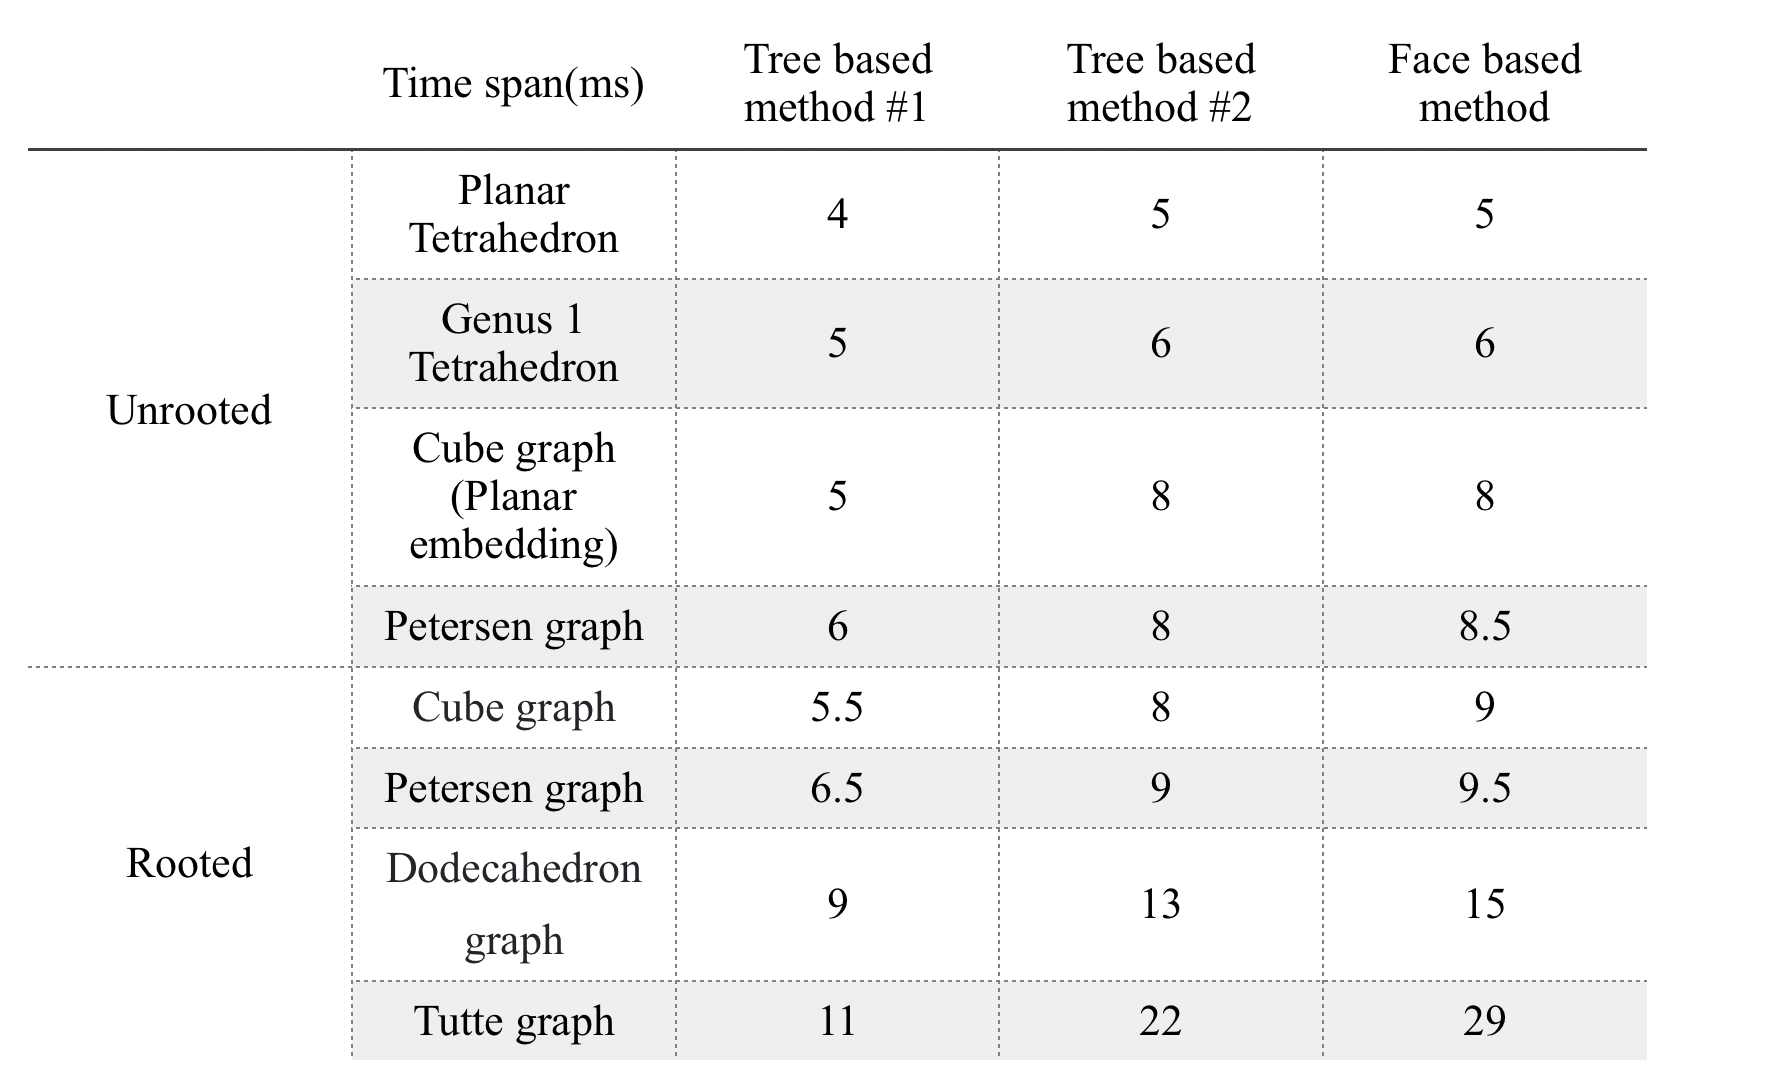
\includegraphics[width=1\textwidth]{../../image/timeconsume.png}
    \caption{The time consuming of the methods for different maps.}
    \label{fig:figures:timeconsume}
  \end{figure}
  We just test this features of each approach on the examples, cause the time for the same method might be a little different for each running. In order to maintain the accuracy of the results, the consequence comes from the average of 10 times testing with the same map. From the result, first tree based method use the least time.  The time span of the improved tree based method and the faces based method almost the same, but the later method spends more time.

  \subsection{Clarity}
  The requirement of the clarity for a visualising result is that users can analysis the output directly and the edges should not be cramped together and have an explicit identity. Firstly, trying a simple combinatorial map whose darts number is 8. Every drawing results of the map is tidy and transparent.
  \begin{figure}[htb]
    \centering
    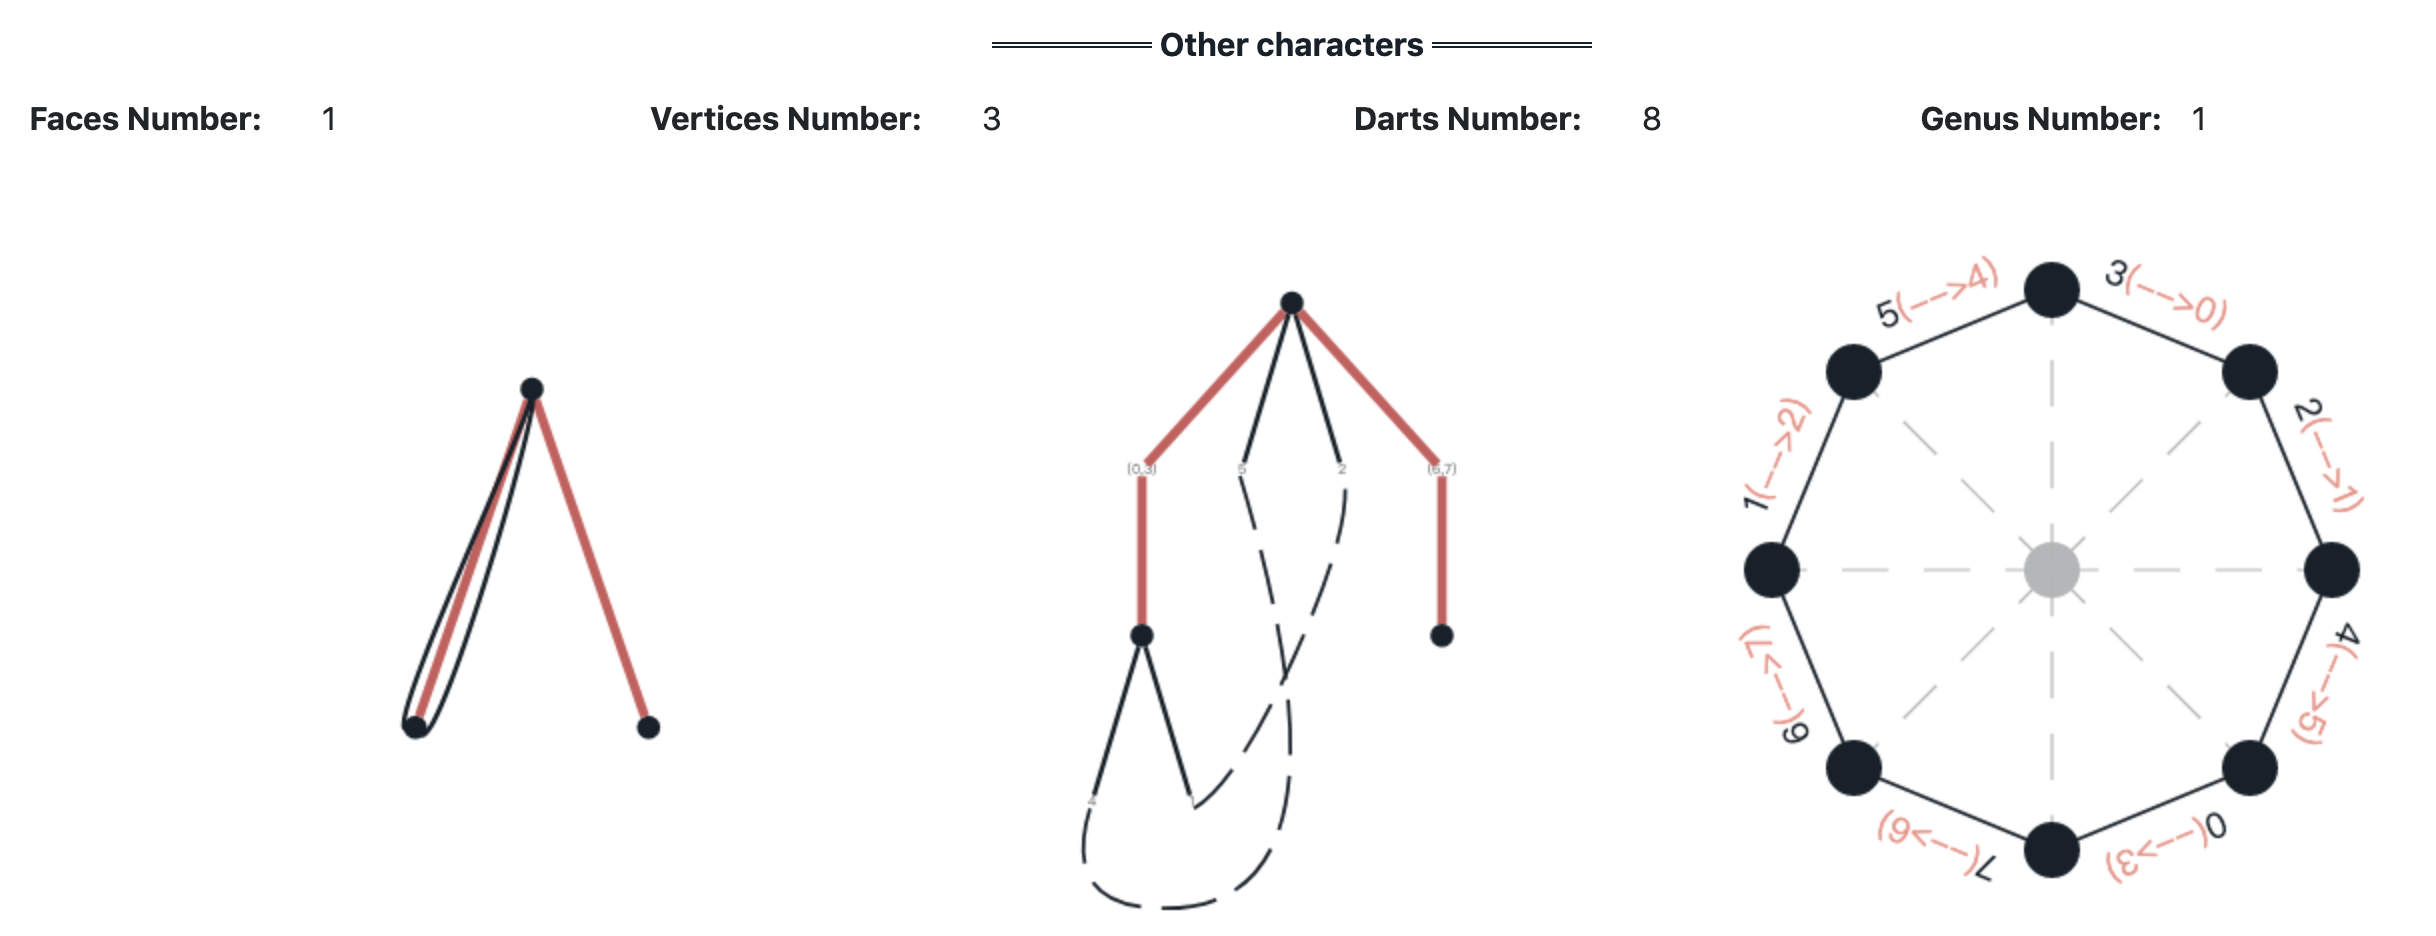
\includegraphics[width=1\textwidth]{../../image/clear1.png}
    \caption{A random map with 8 darts.}
    \label{fig:figures:clear1}
  \end{figure}

  Drawing a larger combinatorial maps based on the 100 darts. The edges cramped together and hardly to recognise the structure of the map for the first method. The second method still retain a beautiful and complete structure. The most neat result is the last one.

  \begin{figure}[htb]
    \centering
    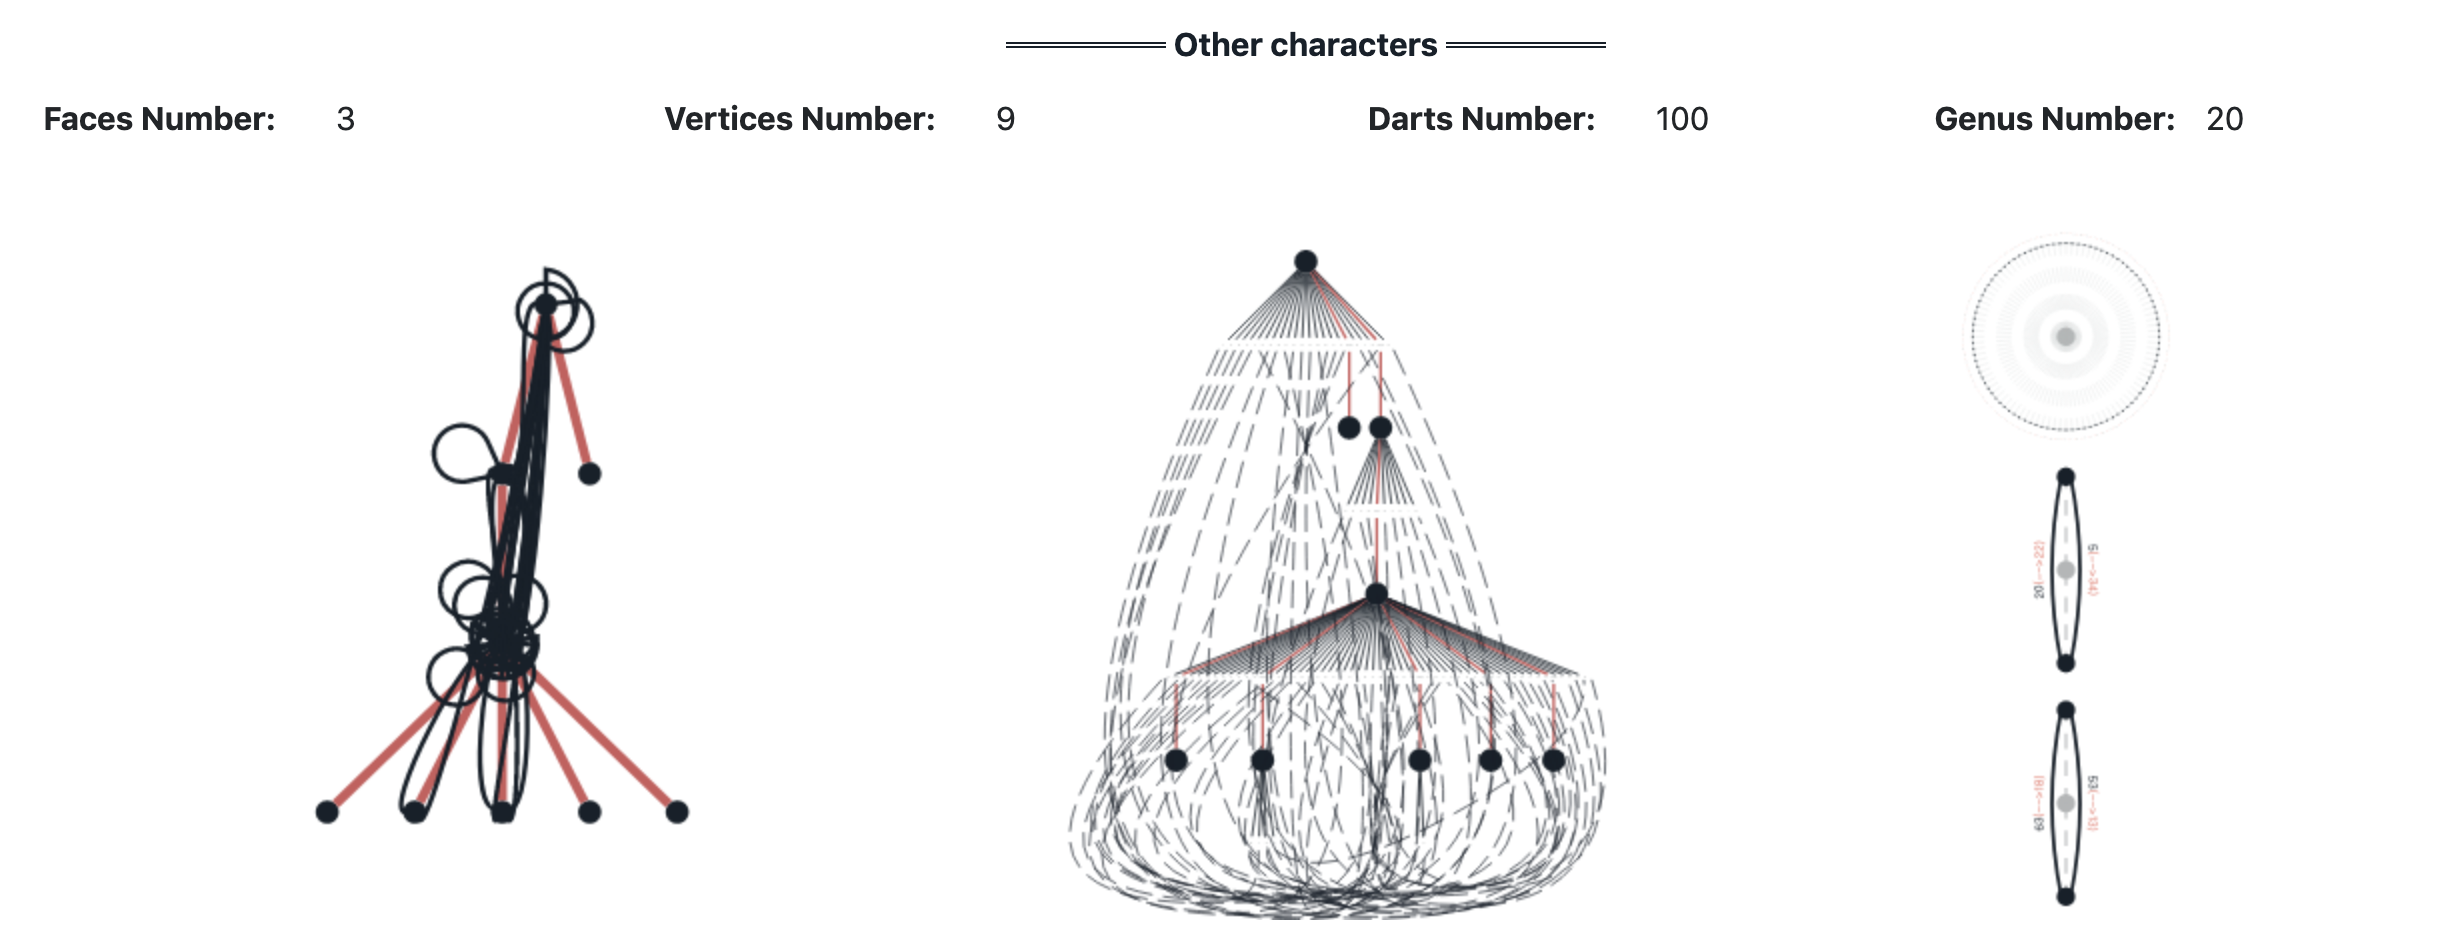
\includegraphics[width=1\textwidth]{../../image/clear2.png}
    \caption{A random map with 100 darts.}
    \label{fig:figures:clear2}
  \end{figure}

  The \cref{fig:figures:clear3} shows a combinatorial map having 1000 darts and 50 vertices. It cannot be recognised any plot of structure, even the tree structure in the first result. The last two still maintain a featly and legible structure. The only one problem for the last method is that it just shows each face and indicates the darts number and the connection information at the darts around the faces. The number is too small to read for  a larger map, and readers cannot joint every faces together.
  \begin{figure}[htb]
    \centering
    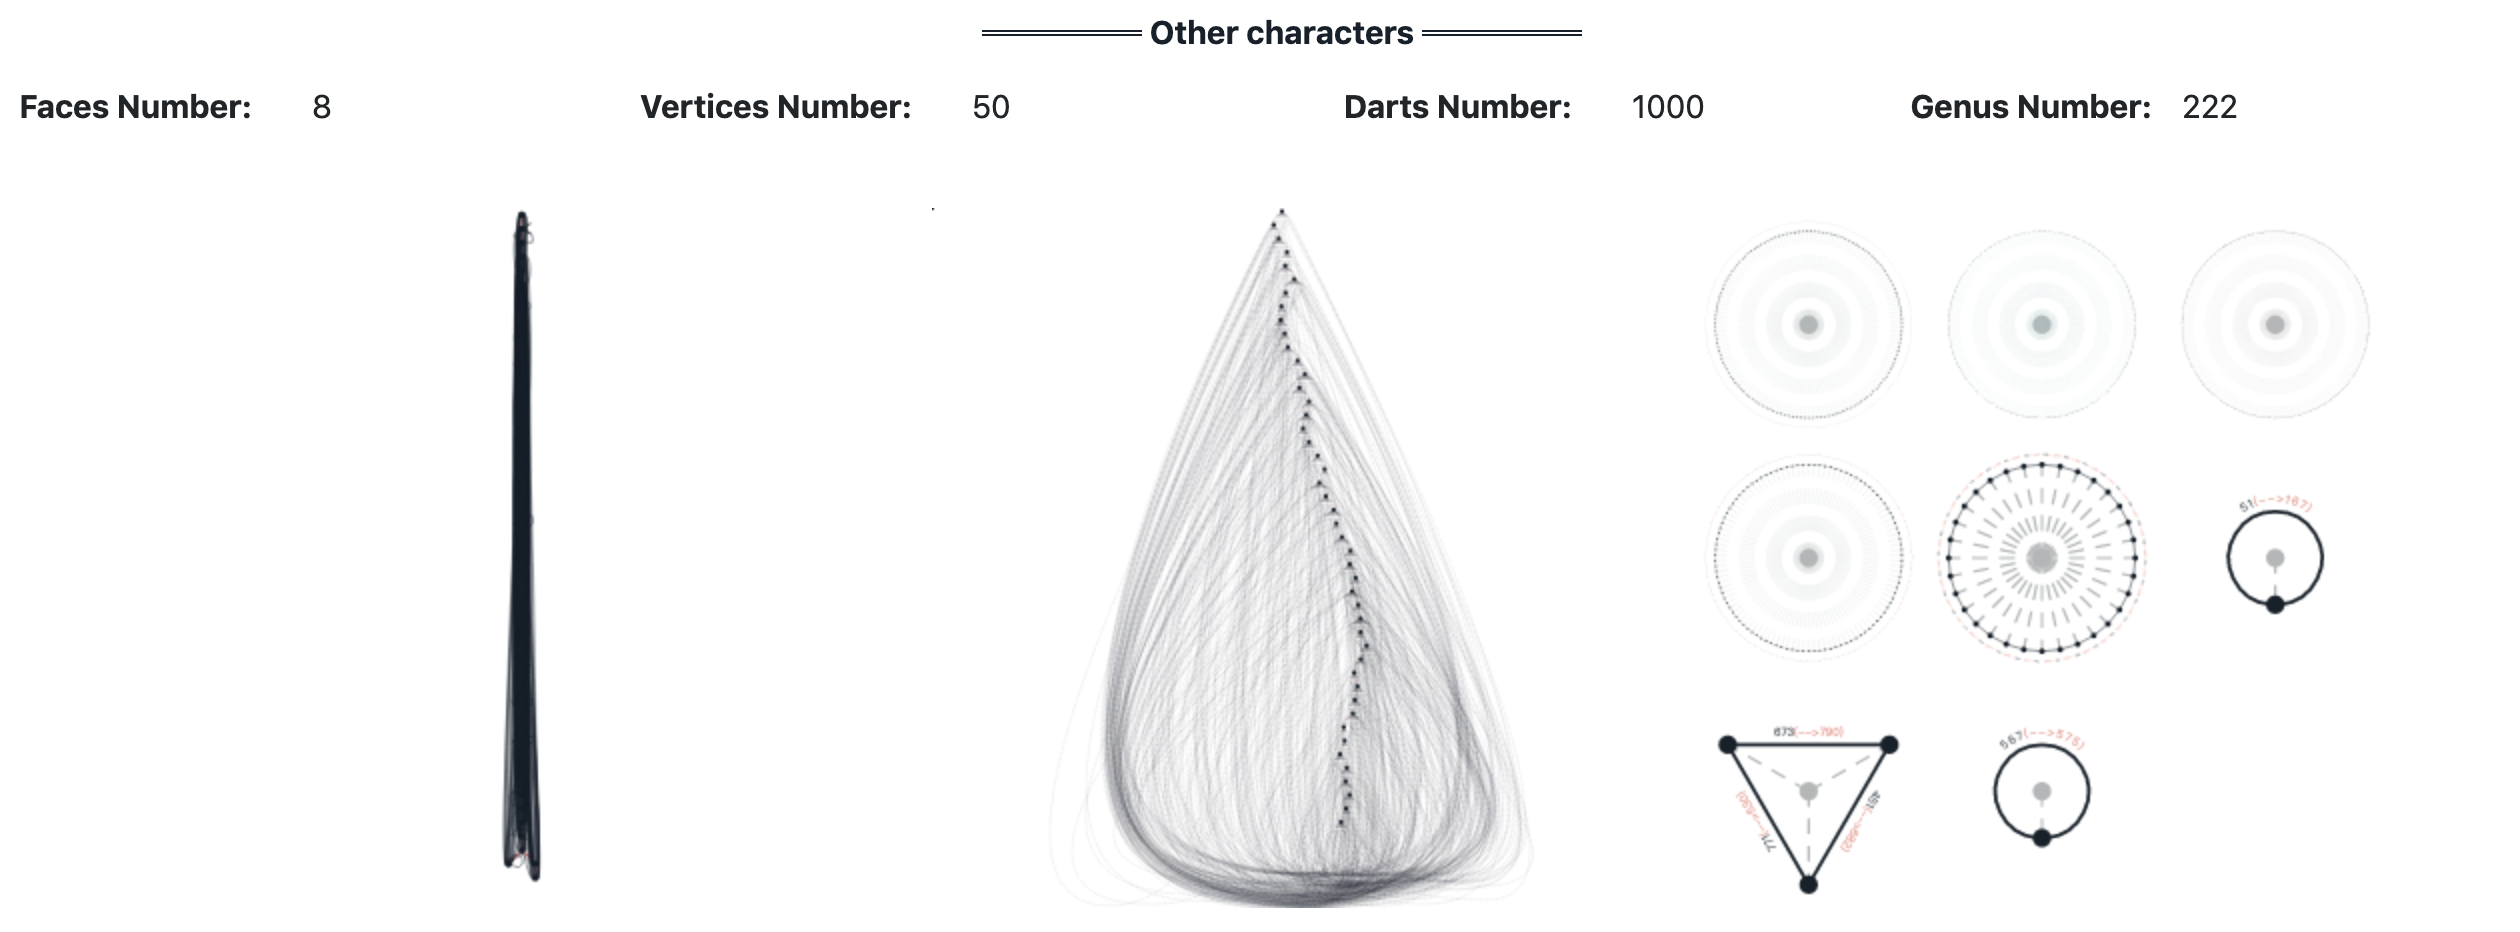
\includegraphics[width=1\textwidth]{../../image/clear3.png}
    \caption{A random map with 1000 darts.}
    \label{fig:figures:clear3}
  \end{figure}

  \subsection{Usability}
  All of the methods can generate a combinatorial maps successfully and the results are correct. For improving the aesthetics problem in first image, the highlight and tips are used to indicate the edges and vertices, though it just an assistant operation without changing the result. The highlight also occurs in the second method, since the edges are so slim that it difficult to spot the specific path of it in a large maps.  The SVG images can be zoomed through clicking the nodes in the them or some other operations with mouse like scrolling the mouse in the space. A reset button is used to recover the whole image.

\section{Testing the system}
After estimate the visualisation approaches, the system should be tested according to whether the specification in chapter 4 is satisfied. This also help to point out the bugs in the current system.

\subsection{Calculating of combinatorial maps}

\subsection*{Parsing the user input which is limited to the cycle notation. All the specifications in this item can be test under the `specific’ tab in the input area.}

\textbf{Correctness} Checked by entering a variety of valid strings, and making sure that the results match the cycle notation for each component. All tests are \textbf{passed}.

\textbf{Reliability} Checked by inputing different types of invalid strings. The error massage and simple examples occurs real time for the illegal string. As the mean time, if click `create’ button when the inputs are illegal, the output will give the corresponding error message rather than continue to generation of the maps. All tests are \textbf{passed}.

\textbf{Performance} Checked the corresponding text and images for a parsing in the output area are correct by hand. The test is \textbf{passed}.

\subsection*{Transforming cycle notation to one-line notation.All the specifications in this item can be test under the `specific’ tab and `random’ tab in the input area.}

\textbf{Correctness} Checked by entering different strings of  these two notations. The output should match the format of another notation. The test is \textbf{passed}.

\textbf{Performance} TChecked the corresponding text and images for a transformation in the output area are correct by hand. The test is \textbf{passed}.

\subsection*{Computation of faces by given the permutations of vertices and edges. This particularly depends on the equation \(\phi=\sigma o\alpha\). All the specifications in this item can be test under the `specific’ tab in the input area.}

\textbf{Correctness} Checked by entering variety vertices and edges permutations. The faces can be conducted in both notations. The test is \textbf{passed}.

\textbf{Performance} Checked the corresponding text and images for a face in the output area are correct by hand. The test is \textbf{passed}.

\subsection*{Generating a random combinatorial map by only given the number of darts (and vertices). All the specifications in this item can be test under the `random’ tab in the input area.}

\textbf{Correctness} Checked by entering different numbers of  darts and generating the graph which is connected successfully. The test is \textbf{passed}.

\textbf{Performance} Checked the text and images for each component in a map in the output area are correct by hand. The test is \textbf{passed}.

\subsection{Visualising combinatorial maps}

\subsection*{The tool using different methods to visualise the combinatorial maps. All the specifications in this item can be test at the bottom of the output area.}

\textbf{Correctness} Checked by judging whether the results of methods followed the constraints of the maps, that is, it must obey the orientation of each part.The whole structure must be connected and filled in the specific area without overflow. For the planar map, it must avoid the crossing as much as possible. All the tests are checked by hand, and the first two tests are \textbf{passed}. For the last test, the last method \textbf{passed}, while, for the first two, it \textbf{failed}.

\textbf{Clarity} Checked by making sure that users can have a clear mind when they look at the images immediately. This test \textbf{passed} for the last two methods and \textbf{failed} for the first approach.

\textbf{Performance} Checked by making sure that it shows the results in the right area and has an effective introduction. These test \textbf{passed}. Checked by creating a map in the limited time. This test \textbf{failed} when generating a large map with the huge number of vertices.

\textbf{Consistency} Checking by making sure the result of the certain method for a map must be the same at any time. These test \textbf{passed}.

\textbf{Aesthetics} Checked by showing tools to they others, and the receiving the feedback of the users. The most feedback is beautiful, colourful and clearly structural for the whole tool, but the result for the first approach looks a little terrible. Therefore, this test \textbf{passed} for the whole structure but \textbf{failed} for a specific result.

\subsection{Knowledge of combinatorial maps}

\subsection*{The tool aims to pass more information about combinatorial maps for whether they are beginners or experts in the relative area.  A introduction of the maps and tool is necessary.}

\textbf{Correctness} Checked by making sure the background of the combinatorial maps is correct and not misleading. The test \textbf{passed}.

\textbf{Performance} Checked whether each section of the introduction displays successfully and is there a introduction at the beginning of the visualiser page. The test \textbf{passed}.
